%%\documentclass{article}
%\usepackage{tikz,pgfplots}
%\usepackage[pdftex,active,tightpage]{preview}
%\begin{document}
%\begin{preview}
%%%%%%%%%%%%%%%%%%%%%%%%%%%%%%%%%%
%%%%%%%%%%%%%%%%%%%%%%%%%%%%%%%%%%%%%%%%%%%%%%%%%%%%%%%%%%%%%%%%%%%%%%%%%%%%%%%%%%%%%%%%%%%%%%%%%%%%
%%% Obtained with ..MATLAB/WideFieldScan/Paper/QualityPlotPaper.m for a SimluationSize of 1000px %%%
%%%%%%%%%%%%%%%%%%%%%%%%%%%%%%%%%%%%%%%%%%%%%%%%%%%%%%%%%%%%%%%%%%%%%%%%%%%%%%%%%%%%%%%%%%%%%%%%%%%%
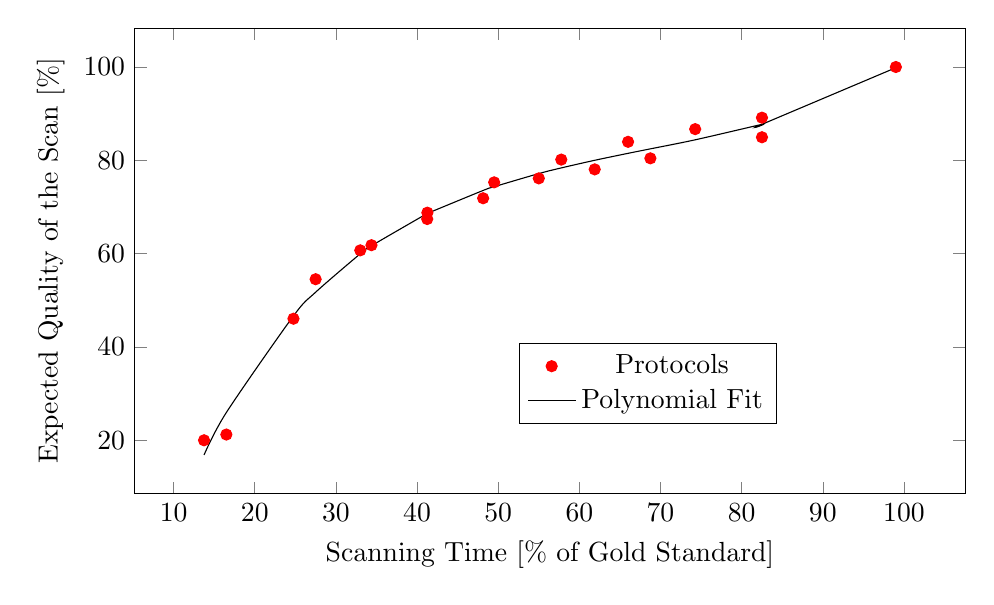
\begin{tikzpicture}

% defining custom colors
\definecolor{mycolor1}{rgb}{0,0.5,0}

\begin{axis}[%
	width=\linewidth,
	height=0.618\linewidth,
%	title={QualityPlot},%
	xlabel={Scanning Time [\%\ of Gold Standard]},%
	ylabel={Expected Quality of the Scan [\%]},%
	]

% Protocols
\addplot [ color = red, only marks, mark = *] 
coordinates{
 (13.7508,20) (16.5009,21.2284) (24.7703,46.0522) (27.5016,54.5201) (33.0019,60.7072) (34.3801,61.8107) (41.2524,67.4167) (41.2712,68.7811) (48.1435,71.8724) (49.5028,75.28) (55.0031,76.1345) (57.7722,80.1592) (61.8943,78.0612) (66.0038,83.9645) (68.7539,80.4284) (74.2731,86.6889) (82.5047,84.9458) (82.5047,89.1421) (99.0057,100)
};

% Line plot
\addplot [smooth, solid]
coordinates{
 (13.7508,16.8548) (16.5009,25.9575) (24.7703,46.6567) (27.5016,51.7347) (33.0019,59.9714) (34.3801,61.6854) (41.2524,68.6146) (41.2712,68.6305) (48.1435,73.5452) (49.5028,74.3455) (55.0031,77.1605) (57.7722,78.3754) (61.8943,80.0091) (66.0038,81.5005) (68.7539,82.4599) (74.2731,84.3973) (82.5047,87.719) (82.5047,87.719) (99.0057,99.8565)
};

\pgfplotsset{every axis legend/.append style={
at={(0.618,0.2)},
anchor=base}}

\legend{Protocols,Polynomial Fit}%$p(x)=p_{1}x^{n}+p_{2}x^{n-1}+...+p_{n}x+p_{n+1}$}

\end{axis}

\end{tikzpicture}
%%%%%%%%%%%%%%%%%%%%%%%%%%%%%%%%%%
%\end{preview}
%\end{document}